% Figure 2: Claw-C Architecture
\documentclass[tikz,border=10pt]{standalone}
\usepackage{tikz}
\usetikzlibrary{arrows.meta,positioning,shapes,calc,fit,backgrounds}

\begin{document}
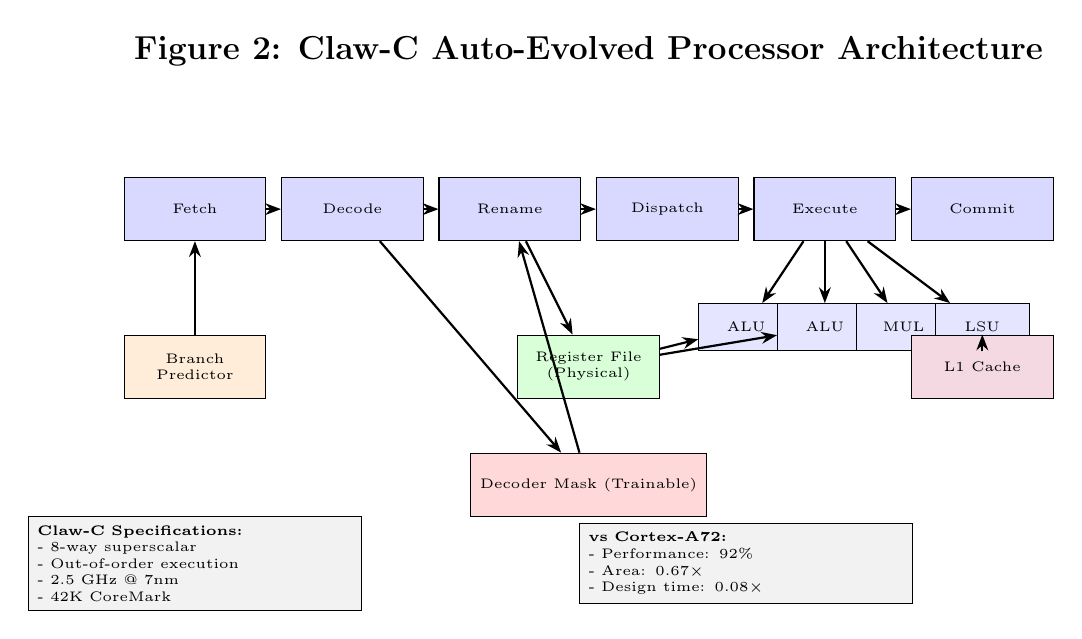
\begin{tikzpicture}[
    node distance=0.8cm,
    block/.style={rectangle, draw, fill=blue!15, minimum width=1.8cm, minimum height=0.8cm, align=center, font=\tiny},
    smallblock/.style={rectangle, draw, fill=blue!10, minimum width=1.2cm, minimum height=0.6cm, align=center, font=\tiny},
    arrow/.style={-{Stealth[length=2mm]}, thick}
]

% Title
\node[font=\large\bfseries] at (0,5) {Figure 2: Claw-C Auto-Evolved Processor Architecture};

% Pipeline stages
\node[block] (fetch) at (-5,3) {Fetch};
\node[block] (decode) at (-3,3) {Decode};
\node[block] (rename) at (-1,3) {Rename};
\node[block] (dispatch) at (1,3) {Dispatch};
\node[block] (execute) at (3,3) {Execute};
\node[block] (commit) at (5,3) {Commit};

% Connections
\draw[arrow] (fetch) -- (decode);
\draw[arrow] (decode) -- (rename);
\draw[arrow] (rename) -- (dispatch);
\draw[arrow] (dispatch) -- (execute);
\draw[arrow] (execute) -- (commit);

% Execution Units
\node[smallblock] (alu1) at (2,1.5) {ALU};
\node[smallblock] (alu2) at (3,1.5) {ALU};
\node[smallblock] (mul) at (4,1.5) {MUL};
\node[smallblock] (lsu) at (5,1.5) {LSU};

\draw[arrow] (execute) -- (alu1);
\draw[arrow] (execute) -- (alu2);
\draw[arrow] (execute) -- (mul);
\draw[arrow] (execute) -- (lsu);

% Register File
\node[block, fill=green!15] (rf) at (0,1) {Register File\\(Physical)};
\draw[arrow] (rename) -- (rf);
\draw[arrow] (rf) -- (alu1);
\draw[arrow] (rf) -- (alu2);

% Branch Predictor
\node[block, fill=orange!15] (bp) at (-5,1) {Branch\\Predictor};
\draw[arrow] (bp) -- (fetch);

% Memory
\node[block, fill=purple!15] (l1) at (5,1) {L1 Cache};
\draw[arrow] (lsu) -- (l1);

% Decoder Mask
\node[block, fill=red!15, minimum width=3cm] (dm) at (0,-0.5) {Decoder Mask (Trainable)};
\draw[arrow] (decode) -- (dm);
\draw[arrow] (dm) -- (rename);

% Statistics box
\node[draw, fill=gray!10, align=left, font=\tiny, text width=4cm] at (-5,-1.5) {
    \textbf{Claw-C Specifications:}\\
    - 8-way superscalar\\
    - Out-of-order execution\\
    - 2.5 GHz @ 7nm\\
    - 42K CoreMark
};

% PPA box
\node[draw, fill=gray!10, align=left, font=\tiny, text width=4cm] at (2,-1.5) {
    \textbf{vs Cortex-A72:}\\
    - Performance: 92\%\\
    - Area: 0.67$\times$\\
    - Design time: 0.08$\times$
};

\end{tikzpicture}
\end{document}
